
%{\normalfont\initfamily \fontsize{12mm}{12mm}\selectfont D}


\cappar Tal como se diz, não basta estudar, é necessário saber aprender; diz-se também: Não basta ensinar, é necessário saber transmitir conhecimentos, hábitos ou habilidades.
\vspace{0.5cm}
\begin{wrapfigure}{r}{0.40\textwidth} 
  \vspace{-55pt}
  \begin{figurebox}
   \vspace{20pt}
    \centering
    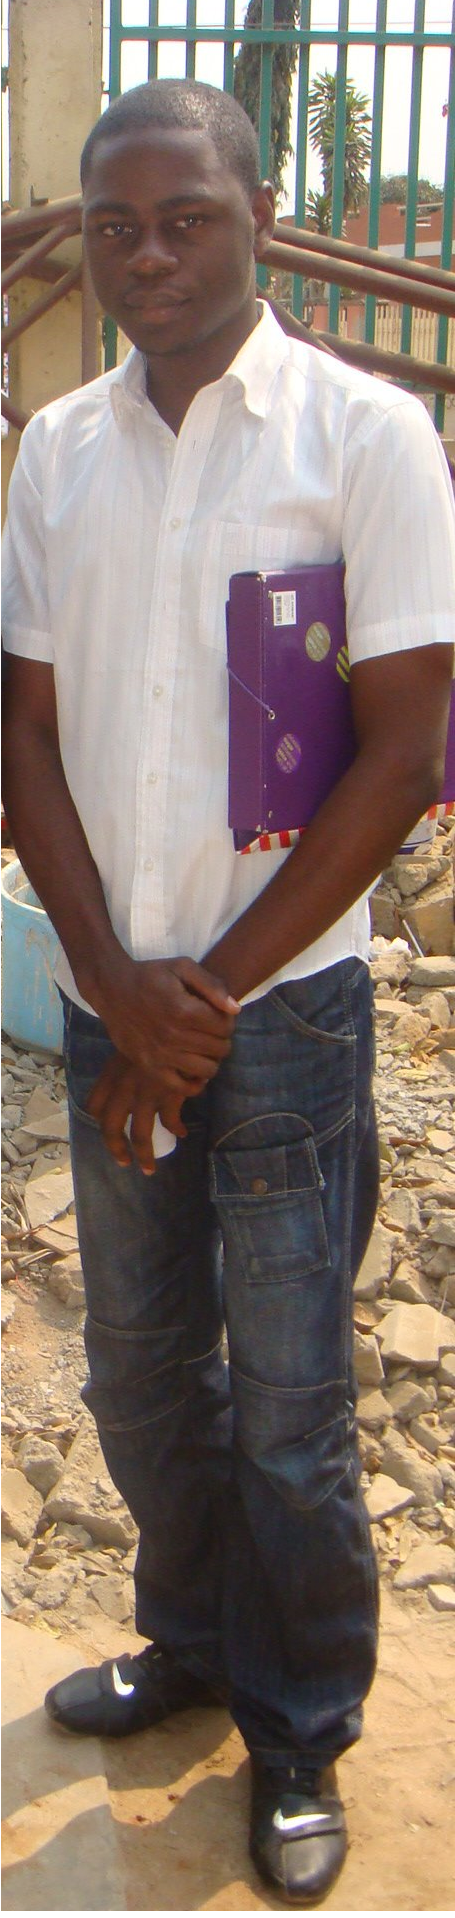
\includegraphics[height=0.75\textheight]{hbc.png}\\
    Hamilton Cristóvão\\ 
     {\sl\small Engenheiro de telecomunicações e professor de Matemática}
    \vspace{1pt}
    %\vspace{0.1\textheight}
  \end{figurebox}
 \vspace{-20pt}
\end{wrapfigure}

\section{Ensino em Angola}
Angola é um país em via de desenvolvimento, vem de longos anos de conflito armados: (1975-2002). Aspecto que contribuiu bastante para uma educação académica debilitada, por factores sócio-económicos sobretudo.

Temos deficit tanto a nível de docência como no lado discente, onde muitas vezes o conhecimento dos alunos não é proporcionala  sua classe ou ciclo. Debilidades que são registadas maioritariamente em escolas estatais e colégios periféricos.

Mas tem-se visto o grande esforço do estado em superar esta situação. E por outro lado, temos notado também casos particulares de estudantes até carentes em condições económicas que se têm destacado com aproveitamento excelente, fruto de esforços e/ou pesquisas ou simplesmente por ter passado em “mãos” de bons mestres.

\section{Formação em escolas Católicas}

Falando da minha experiência em escolas Católicas, (que é o maior fundamento de minha metodologia), tive professores Brasileiros, Angolanos, e Espanhóis.

Meu professor de Matemática Brasileiro usava uma metodologia indutiva. Era muito concreto e objectivo na apresentação de um novo conteúdo, as aulas incidiam mais na resolução de exercícios, iniciava com os mais simples possíveis(algumas vezes até troçávamos da facilidade), e no final do tema acabávamos por resolver exercícios complexos mas de uma forma que nos pareciam simples.

A professora Angolana, trabalhava mais com os manuais. Apresentava-nos a matéria de maneira muito fiel aos livros; pela maneira que vinham as avaliações, sobretudo pela linguagem; impulsionava-nos mais a pesquisar exercícios nos livros para evitar as grandes surpresas nas avaliações. Mas foi também uma experiência bastante divertida.

O Professor Espanhol, tinha uma maneira muito científica de ver a matemática(afinal de contas ela é mesmo uma ciência!), ajudou-nos a perceber melhor a linguagem Matemática e toda a sua coerência bem como a aumentar o rigor em nossos trabalhos. Incentivou-nos a procurar os porquês, até mesmo das propriedades e fórmulas. Influenciou-nos a desenvolver o nosso auto-didatismo.


\section{Minha Experiência como professor}

Lecciono há quase 5 anos. Meu professor de Metodologia de Matemática com o qual muito trabalhei em Física, sempre  incentivou-me, dizia que tenho jeito para o ensino (afinal sou filho de uma professora de matemática, de mais de 32 anos de carreira).

Mas na verdade, apenas este é o meu segundo ano que lecciono Matemática, nos restantes leccionei Física. Mas por outra, dizer que tive o privilegio de leccionar em escola pública, onde a realidade do ensino e da forma de aprendizagem é muito diferente da realidade onde me encontro agora(escola Católica. 

Gosto de ensinar a Matemática de uma forma prática e clara(sem rodeios). Estou leccionando 10ªclasse. E sei que muitos alunos vêm mau preparados em temas básicos. Daí que estou procurando dar esta “base” necessária e/ou solidificar para os que já têm-na.
Logo após ensinar um novo tema, resolvo alguns de exemplo, e deixo eles resolverem os outros em seus cadernos individualmente, depois de um tempo vou passando nos cadernos para apoiar os que tiverem necessidade ou dificuldade.

Quando o tempo disponível ter passado, permito que um aluno voluntário resolva e explique no quadro. Se o tempo for curto, faço eu mesmo. Mas em geral, em minhas aulas 80\% do tempo disponível, são os alunos a trabalharem, e apenas 20\% estou explicando de forma resumida as ideias dos conteúdos. 

Procuro transmitir o máximo de autoconfiança aos meus alunos, tirando-os o medo de errar e incentivo-os a estudar e perceber bem o que se está fazendo (Qual é a ideia básica do exercício). Em geral quando estou explicando algo no quadro, exijo a máxima atenção de todos, faço-o de forma pausada, não muito lenta também, enfatizando bastante a ideia fundamental.

A resolução de problemas acompanha em geral um capítulo, algumas vezes no início, mas em geral no fim dos capítulos. Deixo os alunos resolverem pelos métodos que lhes convém, mas em geral destaco o mais fácil ou o que melhor esteja de acordo ao tema. Algumas vezes temos que recorrer a uso de objectos concretos(quando noto que uma parte da turma não está conseguindo fazer abstracção), como por exemplo: Chamar vários alunos para virem em frentee  eles(literalmente) representarem um elemento, para fazermos  Permutações, Arranjos, ou o que for, se estivermos por exemplo resolvendo problemas de Análise Combinatória; ou outros quais quer de raciocínio.

Outro elemento metodológico que peço aos alunos, é que na resolução de exercícios façam desenhos ilustrativos do que estão fazendo.

Uma grande dificuldade que tive na escola pública, era assegurar que aprendessem a longo prazo. Quer dizer: ensinava por exemplo hoje o jogo de sinais(até inventei uma música!!!), mas dia seguinte, ou semana seguinte, vários esqueciam… Felizmente em geral na escola Católica é de certa forma diferente. Mas esta era uma realidade difícil. Tive que insistir até ao final do ano.  Mas só no ano seguinte notei efectivamente uma melhoria quantitativa.

Esta é basicamente uma panorama do ensino da Matemática em Angola, baseada em minha experiência.




\newpage
%%% Local Variables: 
%%% mode: latex
%%% TeX-master: "nadaesimposible"
%%% End: 


